%% implemen.tex
%% $Id: implemen.tex 61 2012-05-03 13:58:03Z bless $
%%

\chapter{Implementierung}
\label{ch:Implementierung}
%% ==============================

Aufgrund der unterstützenden Funktionen, wie das Portieren auf verschiedene Systeme, habe ich mich für die Unity Engine in der Version 2019.3.14f entschieden um Latrunculi digital umzusetzen. Die Erklärung zu Unity befindet sich im Abschnitt \ref{ch:Grundlagen:sec:Unity}. Weiterhin habe ich mich in C\# eingearbeitet und damit die verwendeteten Skripte geschrieben und genutzt. Da ich vorher noch nicht mit Unity und C\# gearbeitet habe, benötigte ich etwas Einarbeitungszeit um den ersten Prototypen zu erstellen.

\begin{figure}[h]
	\centering
	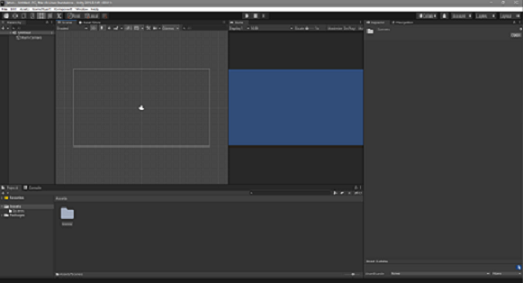
\includegraphics{img/Unity-Editor}
	\caption{Unity-Editor}
	\label{fig:Editor}
\end{figure}

%% ==============================
\section{Unity}
%% ==============================
\label{ch:Implementierung:sec:Unity}

Wie zuvor bereits erwähnt, habe ich die Unity Engine genutzt um das Spiel zu implementieren. Die ersten Versuche einer lauffähigen Umsetzung habe ich mit einem vorgefertigten Spielbrett umgesetzt. Dabei habe ich das Brett durch 8x8 einzelne Zellen beziehungsweise Quadrate dargestellt, die jeweils ein eigenes Spielobjekt sind. Auf diesen Quadraten habe ich die Spielsteine als schwarze und graue Kreise platziert und diesen via Skript Funktionen gegeben. Dieser erste Entwurf \ref{fig:Prototyp} reagierte auf das OnClick() Event, sodass beim Anklicken eines Kreises der mögliche Weg hervorgehoben wurde und beim Klick auf das gewünschte Feld, wurde der Kreis auf diesem neuen Feld platziert.

\begin{figure}[h]
	\centering
	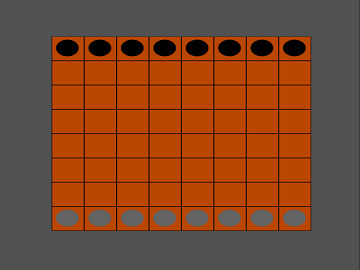
\includegraphics{img/Prototyp}
	\caption{Prototyp}
	\label{fig:Prototyp}
\end{figure}

Da dieser Entwurf sehr statisch und die Größe fest verankert war, habe ich mir Informationen gesucht um das Spiel dynamisch zu erstellen und die Größe des Spielfelds variabel zu machen. Dazu habe ich sowohl für die Zellen, als auch die Spielsteine Prefabs erstellt und somit mittels Skript in der Start-Funktion die Prefabs abrufen und je nach angegebener Größe das Spielfeld zur Laufzeit erstellen.
Außerdem wurde das OnClick()-Event durch Drag \& Drop ersetzt, sodass es auf einem Touchscreen intuitiver zu bedienen ist.
%% ==============================
\section{GameObjects}
%% ==============================
\label{ch:Implementierung:sec:GameObjects}
Um die einzelnen Spielelemente darzustellen, müssen im Unity-Editor erst Spielobjekte (englisch: GameObject) erstellt werden. Die folgenden Objekte wurden dem Spiel hinzugefügt:
\paragraph{Main Camera}
Die Kamera ist zuständig für das Sichtfeld, sodass hier festgelegt werden kann, was innerhalb der Szene sichtbar ist.
\paragraph{Board}
Das \textbf{Board} ist das Objekt, dass das Spielbrett darstellt. Via Prefabs werden dem Board zur Laufzeit die einzelnen Zellen hinzugefügt und so das Brett aufgebaut.
\paragraph{PieceManager}
Der \textbf{PieceManager} ist zuständig für die einzelnen Spielsteine, die ebenfalls via Skript und Prefab der Szene und dem PieceManager hinzugefügt werden.
\paragraph{GameManager}
Der \textbf{GameManager} beinhaltet die Spiellogik und lässt das Spiel starten, sowie auch beenden. Hier wird nach jedem Zug geprüft ob ein Spieler gewonnen hat oder das Spiel noch weiter läuft. Weiterhin wird hier die Berechnung der KI angestoßen.
\paragraph{EscapeMenuManager}
Der \textbf{EscapeMenuManager} ist zuständig für das Event-Handling des Menüs und der Buttons. Das heißt, hier wird entschieden, ob das Menü sichtbar und was in dem Menü zu sehen ist.

%% ==============================
\section{Skripte}
%% ==============================
\label{ch:Implementierung:sec:Skripte}
Damit die einzelnen Objekte auch Funktionen und Informationen bekommen, musste jedem Objekt ein Skript hinzugefügt werden.
Beispielsweise hat jeder Spielstein das Skript \textbf{SimplePiece} zugeordnet bekommen. Dieses ermöglicht dem Spielstein die Bewegungen auf dem Spielbrett durchzuführen. Es enthält Funktionen die auf das Ein- und Austreten des Drag\&Drop-Events reagieren. Des weiteren werden hier Informationen über die Ursprungszelle, sowie die aktuelle Zelle gespeichert um das Zurücksetzen des Spiels zu vereinfachen. \\
Das \textbf{PieceManager}-Skript ist für die Spielsteine insgesamt zuständig, das heißt hier werden die Prefabs und Skripte der Spielsteine instanziiert und der Szene hinzugefügt beziehungsweise auf dem Spielbrett platziert. Außerdem kann dieser Manager die Funktionen der Spielsteine ein und ausschalten, sodass nur mit den Steinen interagiert werden kann, die auch gerade am Zug sind, vorausgesetzt das Spiel befindet sich nicht im Simulations-Modus.\\
Der \textbf{EscapeMenuActivator} ist für das Ein- und Ausschalten des Menüs zuständig.\\
Der \textbf{GameManager} stößt jeden Spiel-relevanten Prozess an, speichert ob eine oder zwei KIs aktiviert sind und lenkt dementsprechend das Spielgeschehen. Das Spiel wird hier auch gestartet und beendet.\\
Das Spielbrett erhält das \textbf{Board}-Skript und initiiert den Aufbau des Spielbretts. Außerdem werden hier alle Zellen und deren Anordnung gespeichert, sodass das Board mögliche Züge validieren kann.\\
Für die Berechnungen der KI erbt das Skript \textbf{BoardDraught} die Funktionen und Variablen des Board-Skriptes, übernimmt aber nur die wichtigen Informationen.\\
Jede Zelle erhält ebenfalls ein eigenes Skript (\textbf{Cell}), dass die Position der Zelle beinhaltet und den Spielstein, der sich auf der Position befindet. Außerdem wird hier das Hervorheben der Zellen durchgeführt.\\
Die Klasse \textbf{Move} enthält Informationen für eine mögliche Bewegung, das heißt hier wird die aktuelle Position des gerade betrachteten Spielsteins gespeichert, sowie die Zelle auf welche sich der Stein bewegen kann. Weiterhin enthält diese verschiedene Flags die zur Bewertung der Aktion dienen.\\
Im \textbf{AIManager} befindet sich der MiniMaxing-Algorithmus, der die Berechnungen und Bewertungen der möglichen Züge durchführt. Wie genau der Algorithmus funktioniert wird im nachfolgenden Abschnitt erklärt.

%% ==============================
\section{MiniMaxing}
%% ==============================
\label{ch:Implementierung:sec:MiniMaxing}
Für die Implementierung des MiniMaxing habe ich die Klasse AIManager entworfen. Diese enthält die Funktion Minimax, die das aktuelle Spielbrett als Board, die maximale Suchtiefe, die aktuelle Tiefe und den Spieler der am Zug ist annimmt. Die Berechnungen und Evaluation der möglichen Züge werden anschließend hier rekursiv durchgeführt und es wird die maximal erreichte Punktzahl zurückgegeben, sowie die Referenzierung des zugeordneten Zuges.\\

\begin{lstlisting}
public static float Minimax(
BoardDraught board,
int player,
int maxDepth,
int currentDepth,
ref Move bestMove)
{
	if (board.IsGameOver() || currentDepth == maxDepth)
	{
		board.SetCurrentMove(bestMove);
		return board.Evaluate(player);//board.Evaluate(player);
	}
...
}
\end{lstlisting}

Der Algorithmus beginnt mit der Prüfung, ob das Spiel beendet ist oder die maximal festgelegte Suchtiefe erreicht wurde. Trifft einer der beiden Fälle zu, dann wird die Punktzahl des aktuell betrachteten Zuges zurückgegeben, ansonsten wird die Abfrage übersprungen und es geht weiter im Code.\\

\begin{lstlisting}
public static float Minimax(...)
{
		...
	bestMove = null;
	float bestScore = Mathf.Infinity;
	if (board.GetCurrentPlayer() == player)
	bestScore = Mathf.NegativeInfinity;
	List<Move> allMoves = new List<Move>();
	int nextPlayer = 0;

	if (player == 2)
	{
		allMoves = board.GetMoves(player);
		nextPlayer = 1;
	}
	else if (player == 1)
	{
		allMoves = board.GetMoves(player);
		nextPlayer = 2;
	}
	BoardDraught bTest = board;
	Move currentMove;
	if (currentDepth == 0)
	{
		float maxScore = 0;
	}
		...
}
\end{lstlisting}
Anschließend werden die möglichen Züge des gerade betrachteten Spielers berechnet. Dabei wird die Funktion GetMoves(player) aus der BoardDraught-Klasse aufgerufen, die die entsprechenden Züge als Liste zurückgibt.\\
\begin{lstlisting}
public static float Minimax(...)
{
	...
	foreach (Move m in allMoves)//board.GetMoves())
	{
		bTest = board.MakeMove(m);
		float currentScore;
		currentMove = m;
		if (m.attacked)
		{
			if (nextPlayer == 2)
			nextPlayer = 1;
			else
			nextPlayer = 2;
		} 
		currentScore = Minimax(bTest, nextPlayer, maxDepth, currentDepth + 1, ref currentMove);
	...
	}
...
}
\end{lstlisting}

In der Schleife werden die vom aktuellen Zustand machbaren Züge betrachtet und entsprechend wieder die Minimax-Funktion aufgerufen um die Rekursion zu starten. Falls der gerade betrachtete Zug einen Spieler angegriffen hat, wird der Spieler beibehalten um die zweite Bewegung des Spielers ebenfalls zu betrachten.\\

\begin{lstlisting}
public static float Minimax(...)
{
	...   
    board.SetCurrentMove(m);
	float newScore = board.Evaluate(player);
	if (board.GetCurrentPlayer() == player)
	{
		currentScore += newScore;
	
		if (currentScore > bestScore)
		{
			bestScore = currentScore;
			bestMove = m;
			m.mScore = bestScore;
		}
	}
	else
	{
		currentScore -= newScore;
		if (currentScore < bestScore)
		{
			bestScore = currentScore;
			bestMove = m;
			m.mScore = bestScore;
		}
	}
	bTest.StepBack();
	}
	...
}
\end{lstlisting}
Die aktuelle Bewegung wird auf dem Board zwischengespeichert um den Schritt für weitere Evaluationen rückgängig machen zu können. Anschließend wird die Bewegung evaluiert und die Punktzahl entweder auf die Gesamtpunktzahl addiert oder subtrahiert, je nachdem welcher Spieler betrachtet wird. Zum Schluss wird die Bewegung rückgängig gemacht und es kann der nächste Zug betrachtet werden. Nach der Rekursion sollten alle Aktionen eine Bewertung erhalten haben.\\

\begin{lstlisting}
public static float Minimax(...)
{
	...  
	List<Move> bestMoves = new List<Move>();
	if (currentDepth == 0)
	{
		foreach (Move m in allMoves)
		{
			if (m.mScore == bestScore)
			{
				bestMoves.Add(m);
			}
		}
		System.Random rnd = new System.Random();
		
		int index = rnd.Next(bestMoves.Count);
		bestMove = bestMoves.ToArray()[index];
	}
return bestScore;
}
\end{lstlisting}

Da die Punktzahl teilweise identisch war, wurde immer der erste betrachtete Zug mit der maximal erreichten Punktzahl gewählt. Daher habe ich noch einen Zufallsgenerator implementiert, der eine zufällige Bewegung aus denen mit der höchsten Punktzahl auswählt und zurückgibt.


%%% Local Variables: 
%%% mode: latex
%%% TeX-master: "thesis"
%%% End: 
